\section{Конструкторская часть}
\subsection{IDEF0}
Концептуальная модель разрабатываемого компилятора в нотации IDEF0 представлена на рисунке \ref{fig:idef0}.

\begin{figure}[h]
	\begin{center}
		{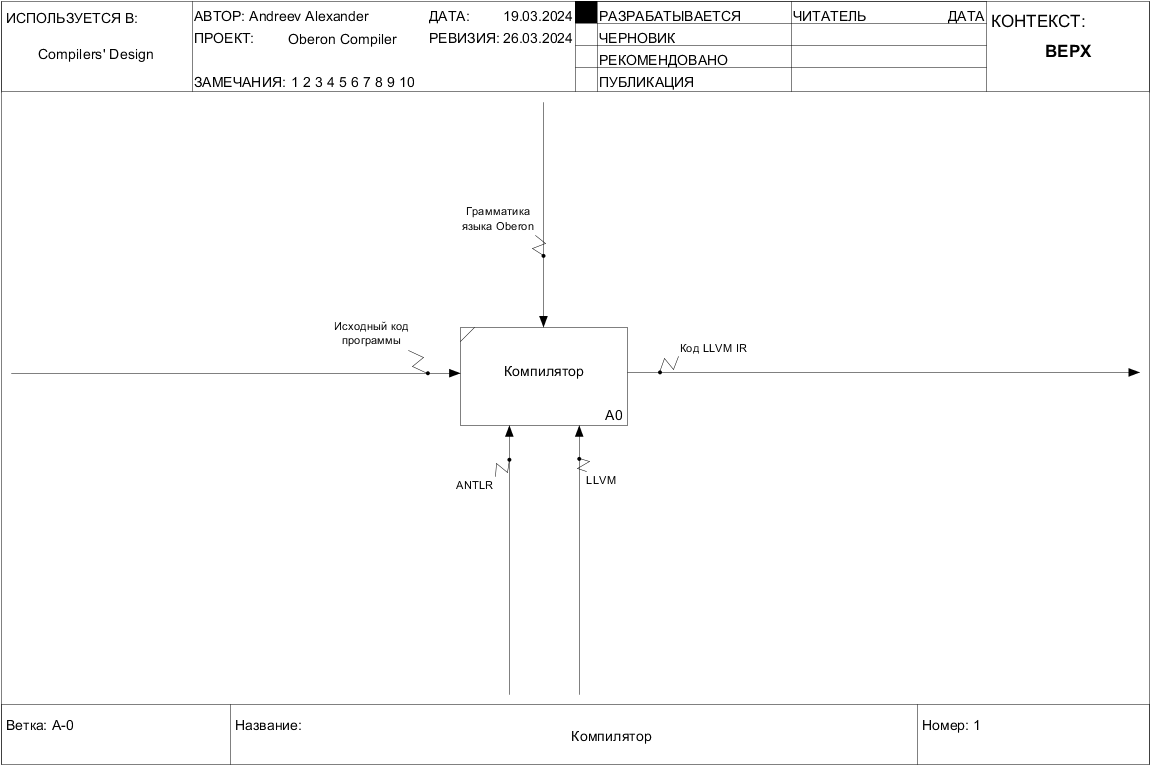
\includegraphics[scale = 0.8, page=1]{img/idef0/01_A-0.pdf}}
		\caption{Концептуальная модель в нотации IDEF0.}
		\label{fig:idef0}
	\end{center}
\end{figure}

\subsection{Язык Oberon}
Oberon -- язык программирования высокого уровня, предназначенный для исполнения программ на одноимённой операционной системе и основанный на таких языках, как Modula-2, Pascal. 

Грамматика приведена в Приложении А. \\

\subsection{Лексический и синтаксический анализаторы}
Лексический и синтаксический анализаторы в данной работе генерируются с помощью ANTLR. На вход поступает грамматика языка в формате ANTLR4 (файл с расширением .g4). 

В результате работы создаются файлы, содержащие классы лексера и парсера, а также вспомогательные файлы и классы для их работы. Также генерируются шаблоны классов для обхода дерева разбора, которое получается в результате работы парсера.

На вход лексера подаётся текст программы, преобразованный в поток символов. На выходе получается поток токенов, который затем подаётся на вход парсера. Результатом его работы является дерево разбора.

Ошибки, возникающие в ходе работы лексера и парсера, выводятся в стандартный поток ввода-вывода. \\

\subsection{Семантический анализ}
Абстрактное синтаксическое дерево можно обойти двумя способами: применяя паттерн Listener или Visitor. 

Listener позволяет обходить дерево в глубину и вызывает обработчики соответствующих событий при входе и выходе из узла дерева. 

Visitor предоставляет возможность более гибко обходить построенное дерево и решить, какие узлы и в каком порядке нужно посетить. Таким образом, для каждого узла реализуется метод его посещения. Обход начинается с точки входа в программу (корневого узла). \\

\subsection*{Выводы}
В текущем разделе была представлена концептуальная модель в нотации IDEF0, приведена грамматика языка Oberon, описаны принципы работы лексического и синтаксического анализаторов и идея семантического анализа.
